\chapter{Event Reconstruction and Monte Carlo Simulations}
After data is collected it is stored in a raw data format.
It can then be used for online reconstruction in the high level trigger
or offline reconstruction. 
In the following section we describe offline event reconstruction;
during this stage a number of algorithms are used to identify and
construct the kinematic properties %%rephrase
of tracks, track vertices,  electrons, muons, taus, jets, missing transverse energy and 
event variables which aid in physics analysis.  
\section{Track and Primary Vertex Reconstruction}
%%%%%%%%%%%%%%%%Track Reconstruction [31] %TRK-11-001
%One of the central design motivations to CMS 
%is a multi-layer tracker with a low occupancy, high granularity
%inner silicon pixel detector and a lower granularity silicon strip detector.
Good track reconstruction provides a means for very accurately determining
the momentum of charged particles.
Identification of the primary vertex, the vertex from
which the signal originates, provides discrimination of the hard scattering process
from pileup vertices.
Furthermore, using tracker tracks to search for secondary vertices
is crucial for accurate identification of heavy flavored jets.
Tracking and vertexing of charged particles is a crucial part of CMS reconstruction
and physics analysis.
\subsection{Track Reconstruction}
\label{sec:TrackReco}
%Track selection involves selection of tracks which are 
%consistent with being produced promptly in the primary 
%interaction region by imposing requirements on the 
%maximum value of significance of the transverse impact 
%parameter relative to the beam spot.
Track reconstruction at CMS follows multiple iterations of a track finding sequence.
The sequence consists of seed generation through hit clustering,
track finding via a filtering technique, track trajectory fitting and finally
selection of tracks that pass quality requirements. 
This technique is known as Combined Track Finding (CTF).
In CTF, the first iteration reconstructs tracks that
have the highest quality. Subsequent iterations reconstruct
tracks with gradually less stringent requirements 
to reconstruct tracks which are lower $p_{t}$, have missing hits or which are greatly displaced.
After each iteration of the CTF track reconstruction sequence, the hits
associated with tracks are removed this reduces the combinatorial complexity
and simplifies subsequent iterations in a search for .

The CTF track reconstruction proceeds as follows:
\begin{itemize}
\item First, seeds are generated which provides the initial track candidates.
Charged particles follow helical paths in the magnetic field, therefore, five parameters (including curvature)
are needed to define a trajectory. To determine these five parameters at least
3 hits or 2 hits in the pixel detector and a constraint on the origin of the track trajectory from the beam
spot is required. Seeds are built in the inner part of the tracker
and track candidates are reconstructed outwards. This is due to a finer granularity 
and hence lower occupancy in the center of the pixel detector. Each iteration of CTF
uses independent quality parameters for seeding layers. 
\item Next, track finding is performed based on the Kalman filter method \cite{KalmanFilter}.
Track finding starts by using the seed trajectories to define and then search
for adjacent layers of the detector with a hit. 
%The next step provides the possibility
%of adding an invalid hit in the case where the particle failed to produce a hit.
After successful identification of adjacent layers with valid hits 
the track finding algorithm updates the trajectories of the tracks. 
\item Track fitting then is used to adjust for the possibility of bias added during the track
finding stage. The trajectory is refitted using a Kalman filter and smoother with
a Runge-Kutta propagator that takes into account both material effect and accommodates
for a inhomogeneous magnetic field.
%track selection sets quality flags and discards tracks that fail certain criteria
\item The final step is track selection where tracks are required to pass a number of quality
based selection criteria. 
The selection criteria puts a requirement on a track's number of layers 
with valid hits, the fit-based $\chi^{2}/dof$, and the track's compatibility
with a primary vertex. In addition to these, several requirements are
imposed as a function of track $p_{T}$, $\eta$, and the number of layers
with valid hits. 
\end{itemize}
%The tracks and primary vertices found with this algorithm are known as pixel 
%tracks and pixel vertices, respectively. 
The performance of the track reconstruction
offline software is shown in figure \ref{fig:TrackerPerformance}.
\begin{figure}[t]
  \centering
 \begin{subfigure}[b]{.4\textwidth}
	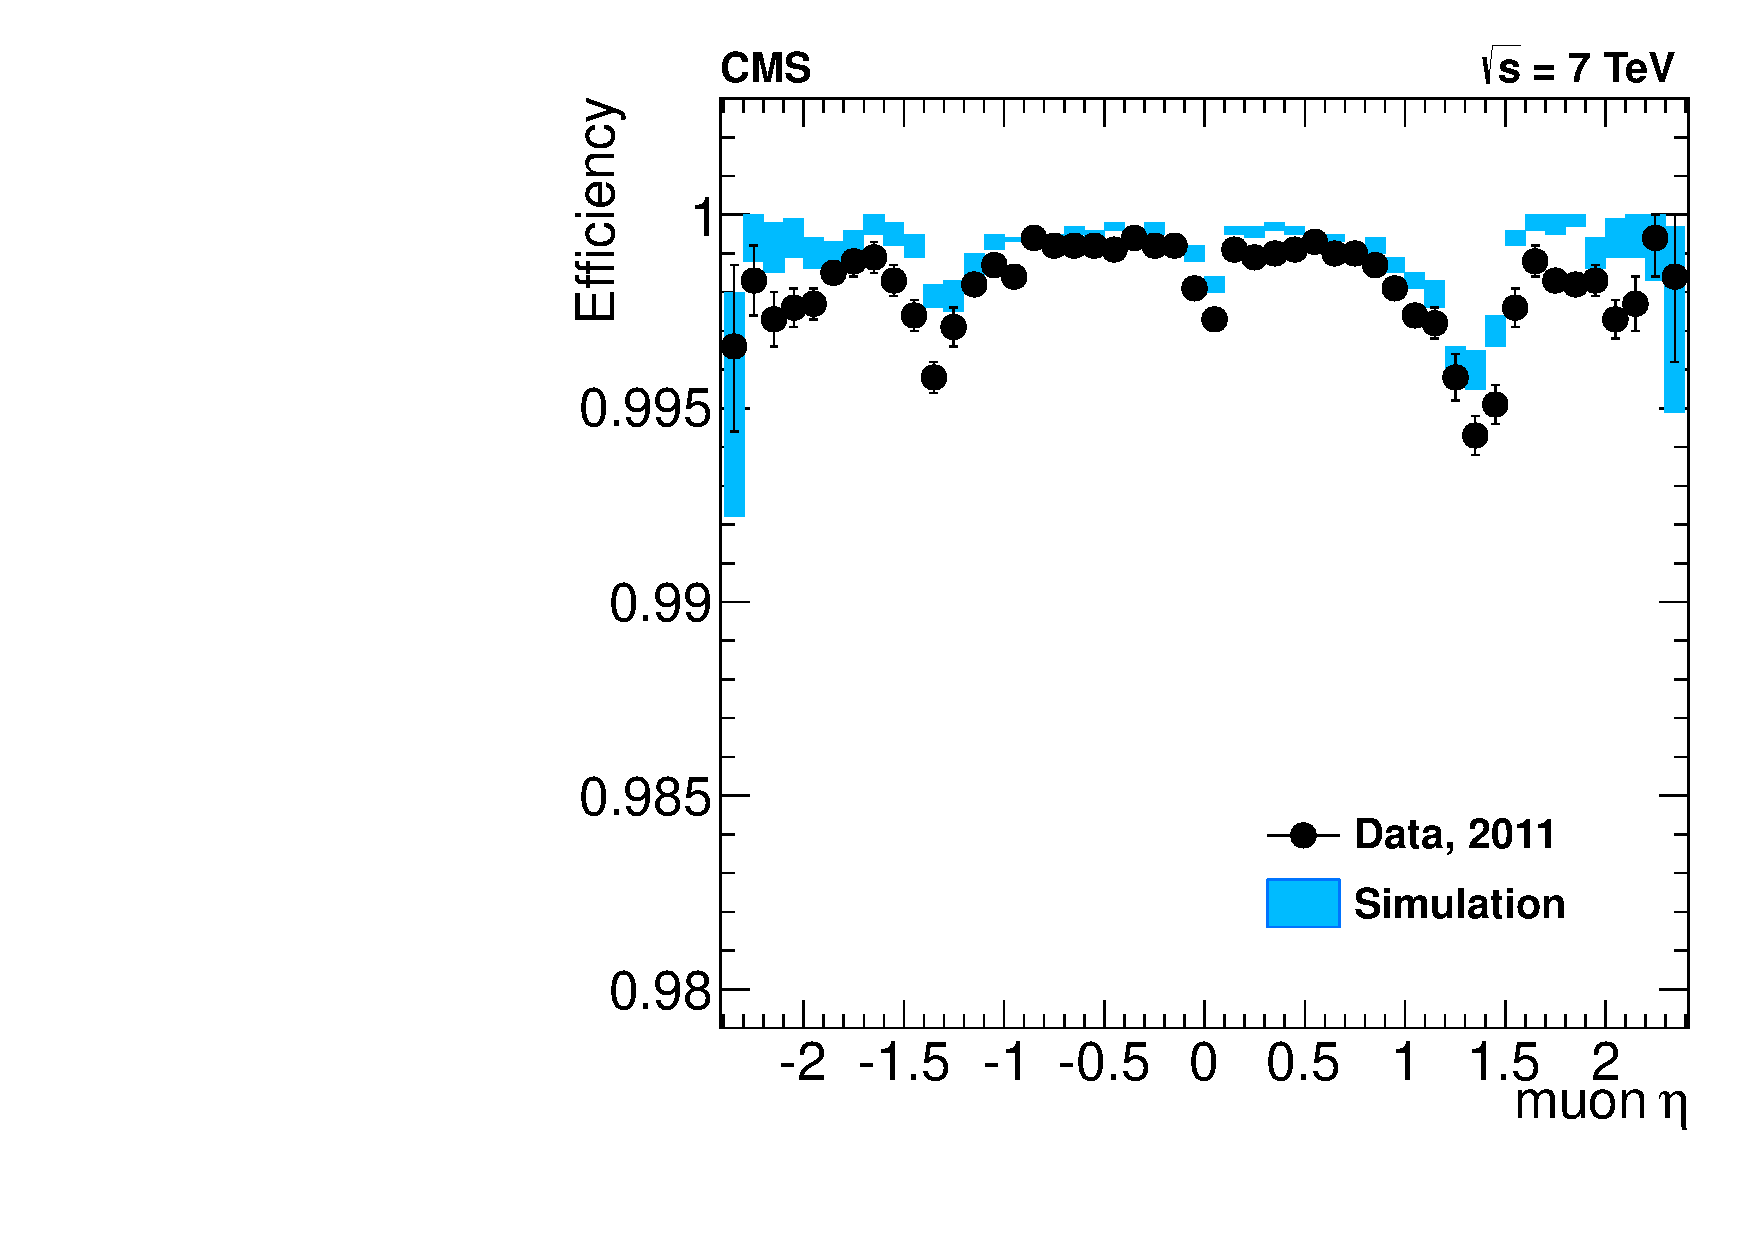
\includegraphics[width=\textwidth]{images/TrackerEffEta.pdf}
  \end{subfigure}
  \begin{subfigure}[b]{.4\textwidth}
	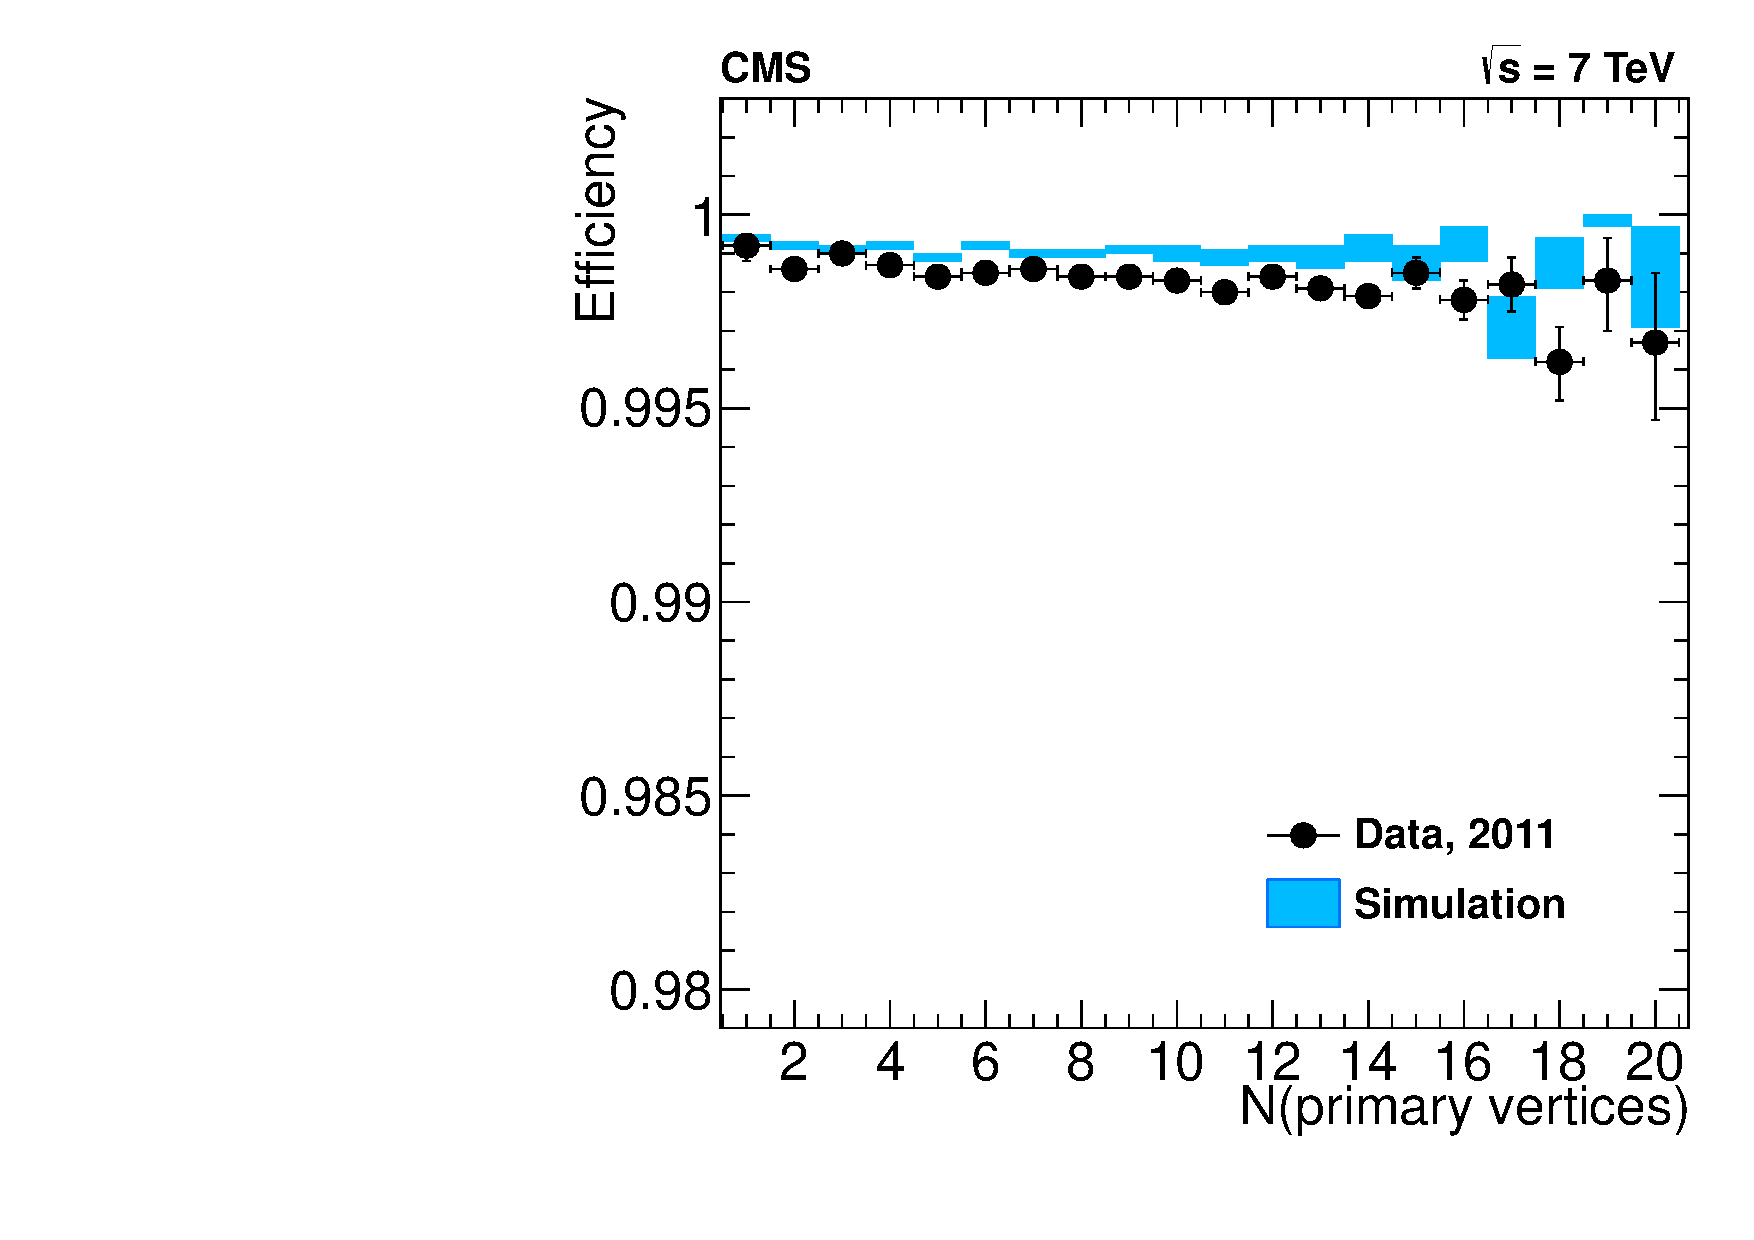
\includegraphics[width=\textwidth]{images/TrackerEffVtx.pdf}
  \end{subfigure}
  	\caption[Tracker Performance]
   	{Tracker efficiency of muons in $Z\rightarrow\mu\mu$ decays. Measured using Tag and Probe as a function of $\eta$ (left) and number of vertices (right)}
	\label{fig:TrackerPerformance}
\end{figure}
\subsection{Primary Vertex Reconstruction}
Primary vertices (PVs) are reconstructed in order to locate and determine the associated uncertainty of all
proton-proton interaction vertices regardless of whether it is a 'signal' or 'background' vertex.
Primary vertex reconstruction proceeds in three steps:
The first step is to select tracks based on their association with a primary interaction region.
To do this, a number of quality selections are imposed: they are based upon the significance of the
transverse impact parameter ($d_{xy}$), the number of strip and pixel hits that are 
associated with a track and the normalized $\chi^{2}$ from the fit to the
trajectory. In selecting tracks, there is no requirement on the $p_{T}$ of the track; 
this is important so that all PVs including ones from minimum bias events are reconstructed.
The second step is to cluster the selected tracks based on their $z$ coordinate at their
point of closest approach to the beam spot. This is done using a Deterministic Annealing (DA)
algorithm which finds a global minimum given many degrees of freedom \cite{DAAnnealing}.
%%More on DA?
The third and final step is to take candidate vertices based on DA clustering in $z$ and use
an 'adaptive vertex fitter' \cite{KalmanFilter} 
to compute vertex parameters. These parameters include the 3-D position and covariance matrix,
as well as indicators for the success of the fit such as the number of degrees ($n_{dof}$) of freedom for
each vertex and weights of the track used in each vertex. The adaptive vertex fitter
uses a modified definition of $n_{dof}$ where,
\begin{equation}
n_{dof} = -3+2\sum^{nTracks}_{i=1} w_{i},
\end{equation}
Here, $w_{i}$ is the weight of the $i^{th}$ track. This implies that $n_{dof}$ is strongly
correlated with the number of tracks that are compatible with arising from the interaction
region which means that $n_{dof}$ can be also be used to select true proton-proton interactions.
For a vertex to be selected at the analysis level, it is required to have a $z$ position
smaller than 24 cm with respected to the origin of the detector, a $\rho$ position
less than 2 cm from the IP and more than 4 degrees of freedom. Of the vertices
that pass this criteria the primary vertex is defined as the one that maximizes
\begin{equation}
\sum_{i} p_{T,i}^{2},
\end{equation}
where the sum extends over all associated tracks and $p_{T,i}$ is the transverse momentum
of the $i^{th}$ track.
\section{Electron ID and Reconstruction}
\label{sec:electronReco}
Electrons in CMS are reconstructed using tracker or ECAL seeds.
Electrons with a low transverse momentum have a higher efficiency
for reconstruction using tracker seeds; whereas electrons with a
higher transverse momentum have a higher efficiency if reconstructed
using ECAL seeds. When traversing the tracker, electrons pass through 
material equivalent to 0.4-0.8 $X_{0}$ 
this causes them to lose a significant portion of 
energy to radiating bremsstrahlung photons. 
This will in turn cause the electron energy deposit to spread in $\phi$. 
Accurate measurement of electron energy 
at the initial interaction point, therefore,
requires collection of photons produced via bremsstrahlung.
%Electron reconstruction is also spread across $\phi$

To begin reconstruction, 
clusters are formed in the ECAL.%, these clusters are then 
%extended in $\phi$ to form super clusters.
Next, electron reconstruction requires
seeds to be produced using either an ECAL driven (1) or a tracker driven approach (2).
(1) is more efficient for electrons with $E_{T}>4$ GeV;
in this method, the clusters produced in the ECAL are
extended in $\phi$ to form super clusters (SCs). 
SCs are then selected and matched back to tracks in the inner tracker layers. 
%The tracker driven approach for electron seeding 
Approach (2) is used to seed
low energy electrons; in this case the energy deposit in the calorimeter
is very broad. All reconstructed tracks are considered as seeds
and the bremsstrahlung hypothesis is tested
by extrapolating a straight line from the track position to the
corresponding ECAL cluster. The process is 
repeated for all layers and a supercluster is defined
by summing all linked electromagnetic cluster deposits. 

Next, trajectories are reconstructed using a dedicated
model of the electron energy loss and fitted using a Gaussian Sum Filter (GSF) algorithm \cite{GSF}. 
The GSF algorithm is preferred over the typical Kalman Filter algorithm.
This choice is motivated by the fact that bremsstrahlung energy loss, 
as described by Bethe and Heitler, 
does not following a Gaussian distribution. 
So, while the Kalman Filter algorithm is optimal in cases where all probability
densities encountered during track reconstruction are Gaussian,
the GSF algorithm distributions are weighted sums of Gaussians and
appropriately describes electron energy loss.
The electron trajectory builder constructs all possible trajectories
for a given seed and the best fit is chosen using a $\chi^{2}$ approach.
Finally, a trajectory smoother is applied.

To improve the electron selection and reject the large QCD backgrounds in the di-tau analysis a 
Boosted Decision Tree (BDT) based %Ref BDT
approach is used. The training has been performed in two
bins of $p_{T}$ and three bins of $\eta$ as shown in Table~\ref{tab:ElectronID-Thresholds}\@.
The BDT has the following $19$ variables as input:

%been trained on data selecting genuine electron candidates from well reconstructed $Z\to ee$ events and
%mis-identified (fake) electron candidates from $Z$+jets events, from which the electrons, which have
%been used to reconstruct the $Z$ boson candidate have been excluded. 

\begin{itemize}
\item
The normalized $\chi^{2}$ of the common track fit, the number of valid hits in the track fit, the normalized
$\chi^{2}$ of the {\it GSFTrack} fit.
\item
The distance in $\eta$ ($\Delta\eta_{SC}({\rm Track}_{vtx})$) and $\phi$ ($\Delta\phi_{SC}({\rm Track}_{vtx})$)
between the reconstructed super cluster in the calorimeter and the track evaluated at the primary vertex
position, the distance in $\eta$ between the super cluster seed and the track evaluated at the calorimeter
surface.
\item
The cluster shape variables $\sigma_{i\eta,i\eta}$ and $\sigma_{i\phi, i\phi}$, where $i\eta$ ($i\phi$)
indicate the integer label of the electromagnetic calorimeter cell in $\eta$ ($\phi$), the cluster shape
variable $f_{e}=1-e1X5/e5X5$, where $e1X5$ ($e5X5$) indicate the energy deposition in an array of $1 \times 5$
($5 \times 5$) cells in the vicinity of the super cluster seed, the cluster shape variable $R9 = e3x3/E_{SC}$,
where $e3x3$ and $E_{SC}$ indicate the energy in an array of $3 \times 3$ cells in the vicinity of the
super cluster seed and the raw energy of the reconstructed super cluster.
\item
The ratio of the hadronic energy over electromagnetic energy of the super cluster ($H/E$), the ratio of
the super cluster energy over the momentum of the associated track evaluated at the selected primary vertex
($E/P$), the variable $1/E_{e}-1/p_{e}$, where $E_{e}$ and $p_{e}$ indicate the reconstructed energy and
momentum of the electron candidate, the ratio of the electron cluster over the momentum of the associated
track and the ratio of the seed cluster over the associated track, where each time the track momentum
has been evaluated at the surface of the calorimeter.
\item
The ratio of the energy that has been reconstructed in the pre-shower detector over the raw energy of
the reconstructed super cluster. The momentum and $\eta$ of the reconstructed electron candidate.
\end{itemize}

An electron is considered as well identified if the BDT discriminator falls above the thresholds shown
in Table~\ref{tab:ElectronID-Thresholds}\@. In addition the electron candidate is required to have a
distance from the selected primary vertex of $d_{z}<0.1$~cm along the $z$ direction of the experiment
 and $d_{0}<0.02 (0.045)$~cm in the plane perpendicular to $z$ in the $e\mu$ ($\mu\tau_{h}$ / $e\tau_{h}$)
decay channel. Further there should be no missing hits in the inner layers of the pixel detector, no
hits before the selected primary vertex and a vertex fit probability of more than $P>10^{-6}$ to minimize the probability that the electron candidate originates from a photon conversion.
%%%%%%%%%%%%%%%%FIX ME

\begin{table}[!ht]
\begin{center}
\begin{tabular}{|l|c|c|c|}
%\cline{2-4}                                                                                                                                                                
\multicolumn{1}{c}{ }      & \multicolumn{3}{c}{\bf BDT Discriminator Value ($>$)}                 \\
\cline{2-4}
\multicolumn{1}{c|}{ }     & $|\eta|<0.8$      & $0.8 \leq |\eta| < 1.479$  & $1.479 \leq |\eta|$  \\
\hline
$\pt\leq 20$ GeV          & $0.925$           & $0.915$                    & $0.965$              \\
$\pt>    20$ GeV          & $0.925$ & $0.975$          & $0.985$    \\
\hline
\end{tabular}
\caption{
  Thresholds for the BDT discriminator to identify electrons. For electrons with $\pt>20$ GeV the values in braces correspond to the Tight ID working point.}
\label{tab:ElectronID-Thresholds}
\end{center}
\end{table}

% Rejection of Electrons from converted photons [39]

%electron ID ---twiki table

%Electron trigger?? maybe
\section{Muon ID and Reconstruction}
Muons at CMS are reconstructed using information from both the 
tracker and the muon detectors. 
%In Wbb high pt muons
%in h to tautau soft muons used.
%Muon reco [40]
\subsection{Standalone Muon Reconstruction}
Standalone $\mu$ reconstruction uses only tracks from the muon system
to reconstruct tracks using a Kalman filter technique which is seeded
by track segments or Level-1 trigger electronics. Tracks are propagated
in iterative steps taking into account the magnetic field, muon energy loss in the material,
multiple scattering and missing hits in the muon system.
Next a suitable $\chi^{2}$ cut is applied to reject bad hits due to showering,
delta rays and pair production. A backward Kalman filter is then applied,
working from outside in and finally the track is extrapolated to the 
beam-spot and a vertex-constrained fit to the track
parameters is performed.
\subsection{Global Muon Reconstruction}
Global muon reconstruction matches standalone tracks to tracks in the tracking
system. 
Tracks are selected which roughly correspond in momentum and position to 
the standalone muon tracks. This is performed in two steps: First,
tracks are selected in a defined $\eta\times\phi$ region which is centered
on the standalone track. Next, spatial and momentum matching is 
used to select the best matching track. Compatibility of the standalone track and tracker tarck with the
primary vertex is also required. Finally a new 'global track' is created combining
tracker and muon hits; at this stage, no new hits are selected, instead, 
the selected hits are refitted as a global track. If more than one candidate
track pair is matched then the candidate with the best $\chi^{2}$ value
is selected. 
For muons with $p_{T}<200\GeV$ the $p_{T}$ measurement is driven
by the fantastic tracker resoluion, for muons with $p_{T}>200\GeV$,
the global-muon fit can improve the momentum resolution compared
to the tracker-only fit.
In muons with a higher $p_{T}$, as might be found
in the boosted topology of $\Wbb$ it is useful to require that muons
are globally reconstructed.
\subsection{Tracker Muon Reconstruction}
In tracker muon reconstruction, all tracks with $p_{T}>0.5$ GeV
and $p>2.5$ GeV are considered as possible muon candidates. 
Track reconstruction is outlined in Section \ref{sec:TrackReco},
after tracks are reconstructed they are extrapolated to the muon
system taking into account effects due to the magnetic field.
If one muon segment matches the extrapolated track then 
it is defined as a tracker muon.  Where matching requires
the the distance in local $x$ between the segment and the extrapolated
track is less than 3 cm or the pull for local x is less than 4 where
the pull is defined as the difference in the position of the matched segment
and the position of the extrapolated track divided by the sum of 
the uncertainties on the position of the matched segment
and the position of the extrapolated track.
%Muon ID (use old muon plots?) mention muon veto in analysis
%Muon trigger

%\section on PF??
% section on lepton isolation?
\section{$\tau$ ID and Reconstruction}
The $\tau$ lepton's high mass means that the $\tau$ plays a very important
roll in search for the SM higgs boson, and MSSM higgs bosons.
The life time of the $\tau$ is short enough that they decay before reaching the inner
most detector. This short lifetime makes $\tau$ reconstruction particularly challenging;
the solution is to reconstruct the decay products of the $\tau$. 

The dominant hadronic $\tau$ decays ($\tau_{h}$) 
and intermediate any intermediate resonances are 
outlined in Table \ref{tab:decay_modes}. 
These decays consist of one or three charged $\pi$ mesons and up to two $\pi^{0}$ mesons.
This thesis uses the hadron plus strips (HPS) algorithm for the reconstruction of 
$\tau_{h}$'s. %%%%ref tau id paper
\begin{table}[b]
\begin{center}
%\tablesize
\begin{tabular}{|l|c|c|c|}
\hline
Decay mode & Resonance & Mass (MeV) &  Branching fraction (\%) \\
\hline
$\tau^{-}$  $\rightarrow $  $h^{-} \nu_{\tau}$ &  &  & $11.6\%$ \\
$\tau^{-}$  $\rightarrow $  $h^{-} \pi^{0}  \nu_{\tau}$ & $\rho^{-}$ & 770 & $26.0\%$ \\
$\tau^{-}$  $\rightarrow $  $h^{-} \pi^{0}\pi^{0}  \nu_{\tau}$ & $a_{\rm{1}}^{-}$ & 1200 & $9.5\%$ \\
$\tau^{-}$  $\rightarrow $  $h^{-} h^{+} h^{-} \nu_{\tau}$ & $a_{\rm{1}}^{-}$  & 1200 & $9.8\%$ \\
$\tau^{-}$  $\rightarrow $  $h^{-} h^{+} h^{-}\pi^{0}  \nu_{\tau}$ & & & $4.8\%$ \\
      \hline
\end{tabular}
\caption{
   Branching fractions of dominant hadronic $\tau$ decays and mass of any intermediate resonance. 
   }
\label{tab:decay_modes}
\end{center}
\end{table}
The HPS algorithm takes into account photon conversions in the CMS tracker
material. %the electron positron decays will bend in the magnetic field
therefore %the HPS algorithm, say something about PF particles
reconstructs photons into 'strips' which are objects which are built%fix
out of electromagnetic particle particles within a window of size $\delta\eta=0.05$
and $\delta\phi=0.20$. The algorithm starts by centering a strip on the
most energetic electromagnetic particle within the PF jet, next it searches
for other electromagnetic particles within the window. If another electromagnetic
particle is found then the object gets associated with the strip and
the four-momentum is recalculated. This procedure is repeated until no other
particles are found. Strips which satisfy the requirement of $p_{T}^{strip}>1GeV/c$
are finally combined with the charged hadrons to reconstruct individual
$\tau_{h}$ decay modes.

The following decay topologies are considered by the HPS $\tau$ ID algorithm:
\begin{itemize}
\item{\bf Single hadron}
      corresponds to $ h^{-} \nu_{\tau}$
      and $ h^{-} \pi^{0} \nu_{\tau}$ decays
      in which the neutral pions have too little energy to be reconstructed as strips.
\item{\bf One hadron $+$ one strip}
      reconstructs the decay mode $ h^{-} \pi^{0} \nu_{\tau}$
      in events in which the photons from $\pi^{0}$ decay
      are close together on the calorimeter surface.
\item{\bf One hadron $+$ two strips}
      corresponds to the decay mode $ h^{-} \pi^{0} \nu_{\tau}$
      in events in which photons from $\pi^{0}$ decays are well separated.
\item{\bf Three hadrons}
      corresponds to the decay mode $ h^{-} h^{+} h^{-} \nu_{\tau}$.
      The three charged hadrons are required                                                                                                      
      to come from the same secondary vertex.
\end {itemize}

Charged hadrons and strips are required to be contained within a cone
of size $\Delta R=(2.8\GeV/p_{T}^{\tau_{h}})$ where $p_{T}^{\tau_{h}}$ is 
the transverse momentum of the $\tau$ hadron $p_{T}^{\tau_{h}}$ is 
required to match the $(\eta,\phi)$ direction of the original PF jet within
a radius of $\Delta R=0.1$. 
%%four momenta must match decay modes
%50-200 MeV for pi0, 0.3 to 1.3 GeV for \rho
%and 0.8 to 1.5 GeV for $a_{1}$

%%%%Tau Isolation from paper
%%%Tau performance plots

\section{Particle Flow Reconstruction}
In proton-proton collisions, even at energies on the order of a few TeV, 
most stable particles produced have a low $p_{T}$.
At CMS, to identify and reconstruct these stable particles a particle flow (PF) event 
reconstruction technique has been developed \cite{PFT09001}\cite{PFT10003}. PF event reconstruction links 
information %find a better word
about reconstructed tracks and calorimeter deposits
to form object collections of 
electrons, muons, photons, charged and neutral hadrons, HF hadrons and HF EM particles
for each event. These collections can then be used to build taus, Jets, $\MET$
and to quantify lepton isolation and tag jets originating from heavy quarks.

The first step of PF reconstruction is to perform
iterative tracking. Here, tracks are first seeded and reconstructed with tight criteria
where the emphasis is on achieving a low fake rate. 
After a track has been identified its hits in the tracker are removed and successive iterative steps
then loosen track identification criteria.

The second step of PF reconstruction is to produce clusters in the ECAL and the HCAL. 
In this step cluster seeds are produced from local calorimeter cell energy maxima
then topological clusters are grown by combining cells with at least one common side
with a cell already in a cluster. 

The final step in PF reconstruction, is to apply a link algorithm which links
hits in the ECAL, HCAL, tracker and muon system. The link algorithm
begins with the outer most hit in the tracker and extrapolates
first to the 2 layers of the ECAL pre-shower. Next, it searches for topological clusters
in the ECAL that correspond to a maximal depth expected of a typical
electron energy deposit profile. Then, A search for topological clusters in the
HCAL is performed at a depth corresponding to 1 $X_{0}$.
The track is linked to any given depth if the extrapolated position in 
the calorimeter is within cluster boundaries. The cluster can be enlarged by up 
to once cell to account for discontinuities in the detector elements, radiation via
bremsstrahlung or pair production. Finally, a link between a charged-particle
track in the tracker and a muon track in the muon system is established
when a global fit returns an acceptable $\chi^{2}$ value.

After these links have been established PF reconstruction is performed which
can be summarized into three steps. First, Electrons are created using GSF filter,
this is further described in section \ref{sec:electronReco}. After electrons
are reconstructed their tracks and calorimetric deposits are removed. Next, 
PF charged hadrons are constructed by identifying links between tracks in the 
tracker and clusters in the ECAL. If the energy deposit in the ECAL is 
the same as the total $p_{T}$ in the tracker within calorimetric uncertainty a 
PF charged hadron is created. If the energy in the calorimeters is much higher
than a PF photon or a PF neutral hadron might also be created. If the energy in 
the calorimeters is too small then a relaxed search for hits in the muon system
is performed. Finally, remaining clusters of ECAL and HCAL clusters give rise
to PF photons and PF neutral hadrons. Figure %insert PFjet figure
shows relative fractions of charged hadrons, photons, neutral hadrons, electrons,
hf hadrons and em particles in jets.

\section{Jet ID and Reconstruction}
%Anti-Kt algo [43]
Jet clustering algorithms have become a crucial part of %%finish  this

Jet clustering in this thesis is performed using the anti-$k_{T}$ jet clustering algorithm \cite{Cacciari:2008gp}.
%The primary motive behind choosing the Anti-$k_{T}$ algorithm is that it is 
In order to perform %new word
comparisons with perturbative effects in theoretical calculations jet clustering algorithm
must be both infrared and collinear (IRC) safe. %check/expand
The development and subsequent choice of the anti-$k_{T}$ jet clustering algorithm
was stimulated by questions of sensitivity to non-perturbative effects like hadronization
and underlying event contamination. Previously used jet clustering algorithms
such as the $k_{T}$ %ref
and Cambridge/Aachen %ref
jet clustering algorithms were IRC safe, however, they
had the property that soft radiation could provoke irregularities in the boundaries
of final jets. 
Algorithms such as SIScone %ref
that were soft-resilient were not %%% IRC safe?

To perform jet clustering in the anti-$k_{T}$, $k_{T}$ and Cambridge/Aachen jet algorithm
a distance $d_{ij}$ is introduced between PF particles $i$ and $j$ and $d_{iB}$ between
the entitiy and the beam (B). The clustering proceeds by identifying the smallest distances.
If it is $d_{ij}$ the entities $i$ and $j$ are combined. However if it is $d_{iB}$ then $i$ 
is considered a jet and all its entities are removed from the list of PF particles. The procedure
is repeated until no entities are left. The definition of $d_{ij}$ and $d_{iB}$ are,
\begin{equation}
d_{ij}=\mathrm{min}(k_{ti}^{2p},k_{tj}^{2p})\frac{\Delta^{2}_{ij}}{R^{2}}
\end{equation}
\begin{equation}
d_{iB}=k_{ti}^{2p}
\end{equation}
where $\Delta_{ij}^{2}=(y_{i}-y_{j})^{2}+(\phi_{i}-\phi_{j})^{2}$, $k_{ti}$ is the 
transverse momentum, $y_{i}$ is the rapidity and $\phi_{i}$ is the azimuthal angle of 
the particle $i$. 
$k_{T}$ is %%write this in
The case where $p=1$ is the $k_{T}$ algorithm, $p=0$ corresponds to the Cambridge/Aachen
algorithm and $p=-1$ is the anti-$k_{T}$ algorithm.
The effects of each of these algorithms on an event with a few well-separated hard particles
and many soft particles is shown in figure%%%insert antikt figure.
%Jets used in this analysis use R=0.5
%The key feature is that soft particle do not modify the shape of the jet while hard particles do.

%Jet energy corrections [44]
\subsection{Jet Energy Corrections}
Jet energy corrections (JEC)
are applied to improve the accuracy of the jet $p_{T}$ measurement
and to flatten the jet energy response as a function
of~$\eta$ and $p_{T}$~\cite{jme-10-010}.
Jets are required to pass identification
criteria that eliminate jets originating or being seeded by
noisy channels in the calorimeter~\cite{Chatrchyan:2009hy}.
Jets which fall within $\Delta R < 0.5$ from a lepton candidate
are not included in the jet collection.

%Pileup ID
\subsection{b-Jet ID}
%%
The Combined Secondary Vertex (CSV) b-tagging algorithm makes use
of the long lifetime and heavy-flavour of the b-hadrons.
%for both b-jets, it is also required that both b-Jets have atleast one secondary vertex.                                                                                   
The CSV b-tagging algorithm combines the following variables into a single discriminating
variable using a Likelihood ratio technique: secondary vertex mass, multiplicity of charged
particles associated to the secondary vertex, the flight significance associated to the
secondary vertex, the energy of charged particles associated to the SV divided by the energy
of all charged particles associated to the jet, the rapidities of charged particle tracks associated
to the secondary vertex, and the track impact parameter significance exceeding the charm threshold.
This algorithm was tuned
using b, c and non-heavy flavour jets from QCD and top samples and provides extreme discrimination
of heavy and udsg jets. At a b-tagging efficiency of 60$\%$, jets from light quarks can be reduced
by a factor of 100!~\cite{refCSV}.

Secondary vertices are reconstructed inside the jet using the Trimmed Kalman Vertex Finder.
This algorithm begins by taking as input all tracks that are inside of the jet and performing a compatibility fit. It then removes the least compatible track and refits the vertex; this procedure is repeated until
the fit is below a given threshold. The secondary vertex studied in this note is that which has
the greatest significance of flight distance.

\section{Missing Transverse Energy}
Missing transverse energy is defined using PF candidates as.
\begin{equation}%%%add vectors above everywhere
\MET = -\sum_{i} p_{T}
\end{equation}
where $i$ runs over all reconstructed PF candidates. 
To improve the $\MET$ resolution in 
events with jets and neutrinos in the decay products 
which are expected to have a high $\MET$, such as $\Wbb$,
recoil corrections are applied to the $\MET$. MVA 
$\MET$ is used in the search for a MSSM $h\rightarrow\tau\tau$;
MVA $\MET$ aims at improving further the $\MET$
through use of recoil corrections and an MVA which targets the true value of the $\MET$.
These procedures are described in the next sections.
\subsection{Recoil Correction}
Momentum conservation in the transverse plane requires,
\begin{equation}
\MET+q_{T}+u_{T}=0
\end{equation}
%where $\MET$ is the missing transverse energy,
where $q_{T}$ is the vector boson transverse momentum which is measured
in $Z\rightarrow\mu\mu$ events and matched to simulation in $W\rightarrow\mu\nu$.
Finally, $u_{T}$ is the transverse momentum of the hadronic recoil.
\begin{equation}
u_{T}\equiv\sum_{j} p_{j,T},
\end{equation}
where the index $j$ runs over all particles initiating at the interaction point excluding
the vector boson. 

\subsection{MVA MET}
MVA PF $\MET$ is based on a set of multivariate regressions.
The purpose of the multivariate regression is to improve measurement of the $\MET$
in the presence of high pileup.
MVA $\MET$ is computed as a correction to $u_{T}$. This correction
is performed in two steps: %using two bdts
first, compute a correction to the azimuthal angle
of $u_{T}$ by training a BDT with the true hadronic recoil, $-q_{T}$, as the target. Next
 a separate BDT is trained to predict the magnitude of $u_{T}$. This corrected
 $u_{T}$ is then used in equation %%%cite equation with recoil
 to calculate a new MVA $\MET$. %list variables? Do I care? it's an f*ing BDT.
